\documentclass[letterpaper, 11pt]{article}
\usepackage[letterpaper, margin=1.4in]{geometry}
\usepackage{amsmath, amssymb}
\usepackage{graphicx}
\usepackage{verbatimbox}
\usepackage{listings}
\lstset{
 basicstyle=\ttfamily,
 columns=fullflexible,
 frame=single,
 breaklines=true,
%postbreak=\mbox{\textcolor{red}{$\hookrightarrow$}\space}
}
\usepackage{caption}
\usepackage{subcaption}

\author{Group~Houston}
\title{API~Documentation}
\date{}

\setlength\parindent{0pt}

\begin{document}
\maketitle
Command design pattern is used for this game. The objects use the command and observable-observer design patterns to determine what happens when objects meet with each other. Singleton design patterns are used when possible. 
\section{View}
We have a 1000$\times$500 game map and a restart button on the canvas.
\section{Controller}
Controller package includes PacWorldController which will process GET and POST requests and return the JSON representation of all the concrete objects in the PacWorld. The controller creates the dispatch adapter and defines the REST end points\\ 
 
The PacWorldController will load and update objects in the PacWorld. It also a reset and clear game options. Meanwhile, it posts the direction information for the Pacman. In addition, it has an endpoint to get the canvas dimension from the front end.
\section{Model}
The model  package includes: DispatchAdapter, command, strategy and objects.

\subsection{DispatchAdapter}
DispatchAdapter communicates with the model and the view. It contains observer lists and parameters for the game includes:
\begin{itemize}
\item Point dims for the dimension of game map
\item static int score to record the score
\item static int lives to record the lives
\item static int fruitTimer to record the cool down time to generate the fruit
\item static int afraidTimer for the time that Pacman can eat ghosts 
\item static int[][] map to construct the game map.
\end{itemize}

Methods in the DispatchAdapter include: loadObject, resetGame, updateGame, switchDirection, canvasDims:
\begin{itemize}
\item DispatchAdapter is the constructor, it calls initializeMap.
\item setCanvasDims set the dimension of the game map. It has one parameter, Point dims. 
\item initializeGame initializes the game. It will load the game map, initialize the Pacman, ghosts, foods, and timers. It does not take any parameter and it has no returns. 
\item updatePacWorld updates the game canvas. It takes no parameters and has no returns.
\item switchDirection switches the direction of the Pacman. It has one parameter, String body, which is the keyboard information from the front end.
 \end{itemize}
 
\subsection{Command}
The cmd package has an interface IGameObjectCmd, which has an execute method. Every concrete command implements this interface. \\%We have three concrete commands: UpdateCmd, SwitchCmd, CollisionCmd.

\subsection{Strategy}
The strategy package has two interfaces:
\begin{itemize}
\item IUpdateStrategy for single object strategies
\item IInteractStrategy for interaction strategies between objects
\end{itemize}

IUpdateStrategy has two methods:
\begin{itemize}
\item getName return the name of the strategy in a string. It has no parameters.
\item update applies the strategy to an object. It has one parameter AGameObject context and no returns.
 \end{itemize}

IInteractStrategy has two methods:
\begin{itemize}
\item getName returns the name of the strategy in a string. It has no parameters. 
\item interact will apply the interact strategy of the src object to the dest object. It takes two parameters, the first is the src object, the second is the dest object. It has no returns.
\end{itemize}
%For single object strategies, we have GhostPatrol, GhostAttack, GhostRandom, GhostRunAway, and PacmanStraight. For interact strategies, we have PacmanEatFood, PacmanEatGhost, PacmanAvoidWall, PacmanExit, GhostAvoidWall, GhostExit. 

\subsection{Objects}
\begin{figure}[htbp] 
\centering
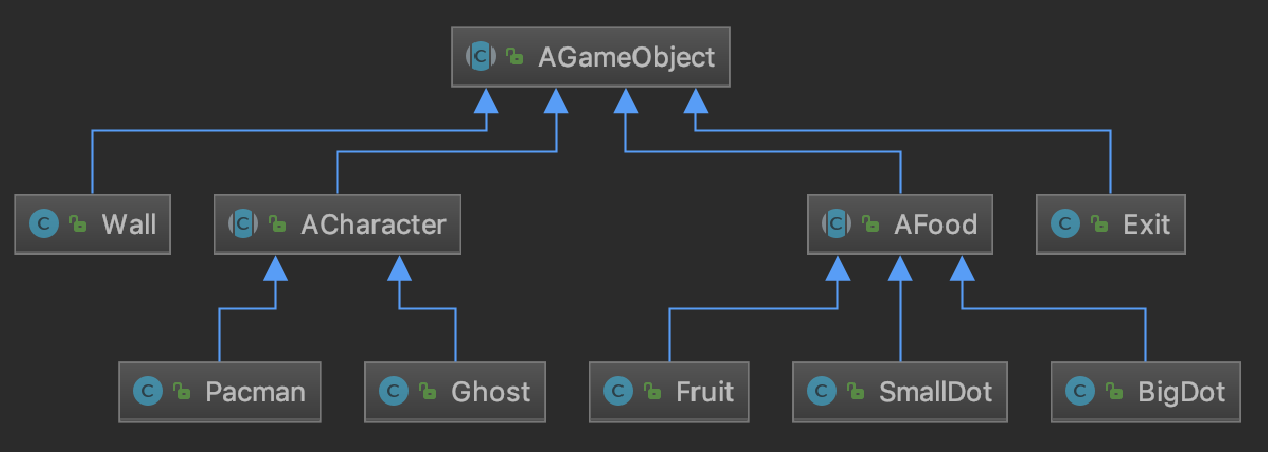
\includegraphics[width=.85\linewidth]{objects.png} 
  \caption{Objects}
  \label{fig1} 
\end{figure}
The object package has an abstract class AGameObject. Two abstract classes ACharater and AFood extend AGameObject. Two concrete objects Wall and Exit extend AGameObject.  Their relationship is shown in figure \ref{fig1}.\\

The AGameObject has a constructor AGameObject, and four methods: getLocation, setLocation, getType, getSize and update. 

\begin{itemize}
\item AGameObject is the constructor, it has three parameters: Point location, String type, int size. 
\item getLocation returns the location of the object in a Point. It has no parameters.
\item setLocation set the location of the object. It has a parameter Point location and it has no returns.
\item getType returns the type of the object in String.
\item getSize returns the size of the object in int.
\item update updates the state of the object using strategies associated with the object.
\end{itemize}

An abstract class ACharacter extends AGameObject for moving objects. Two concrete objects Pacman and Ghost extend ACharacter.  The ACharacter has a constructor ACharacter and six methods: getInteractStrategy, getUpdateStrategy,  setInteractStrategy, setUpdateStrategy, getVel, setVel. 

\begin{itemize}
\item ACharacter is the constructor. It has six parameters: Point loc, String type, Point vel, IUpdateStrategy updateStrategy, IInteractStrategy interactStrategy, int size.
\item getInteractStrategy returns the interact strategy. It has no parameters.
\item getUpdateStrategy returns the update strategy. It has no parameters.
\item setInteractStrategy sets the interact strategy for the ACharacter object. It has one parameter IInteractStrategy interactStrategy and has no returns. 
\item setUpdateStrategy sets the update strategy for the ACharactor object. It has one parameter IUpdateStrategy updateStrategy and has no returns. 
\item getVel returns the velocity of the object in a Point. It has no parameters. 
\item setVel set the velocity of the object. It has one parameter Point vel and has no returns. 
\end{itemize}

An abstract object AFood extends AGameObject for different food. It does not have any new methods. Three concrete objects SmallDot, BigDot and Fruit extend AFood. 

\end{document}